\subsection{Obtaining a Toolchain}

\begin{frame}
  \frametitle{Building a toolchain manually}

  Building a cross-compiling toolchain by yourself is a difficult and painful
  task! Can take days or weeks!
  \begin{itemize}
  \item Lots of details to learn: many components to build, complicated
    configuration. Need to be familiar with building and configuring tools.
  \item Many decisions to make about the components (such as C library,
        gcc and binutils versions, ABI, floating point mechanisms...). Not
	trivial to find working combinations of such components!
  \item Need to be familiar with current \code{gcc} issues and patches
    on your platform
  \item See the {\em Crosstool-NG} \code{docs/} directory for details
    on how toolchains are built.
\end{itemize}
\end{frame}

\begin{frame}
  \frametitle{Get a pre-compiled toolchain}
  \begin{itemize}
  \item Solution that many people choose
    \begin{itemize}
    \item Advantage: it is the simplest and most convenient solution
    \item Drawback: you can't fine tune the toolchain to your needs
    \end{itemize}
  \item Make sure the toolchain you find meets your requirements:
    CPU, endianness, C library, component versions, ABI, soft float
    or hard float, etc.
  \item Possible choices
    \begin{itemize}
    \item Toolchains packaged by your distribution. For example on Ubuntu:
	  \code{sudo apt install gcc-arm-linux-gnueabihf}
    \item Bootlin's GNU toolchains (for most architectures):
          \url{https://toolchains.bootlin.com}
    \item ARM GNU toolchains released by ARM (previously shipped by Linaro):
	  \url{https://tinyurl.com/2fkvvrju}
    \end{itemize}
  \end{itemize}
\end{frame}

\begin{frame}
  \frametitle{Toolchain building utilities}
  Another solution is to use utilities that {\bf automate the process of
  building the toolchain}
  \begin{itemize}
  \item Same advantage as the pre-compiled toolchains: you don't need
    to mess up with all the details of the build process
  \item But also offers more flexibility in terms of toolchain
    configuration, component version selection, etc.
  \item They also usually contain several patches that fix known
    issues with the different components on some architectures
  \item Multiple tools with identical principle: shell scripts or
    Makefile that automatically fetch, extract, configure, compile and
    install the different components
\end{itemize}
\end{frame}

\begin{frame}
  \frametitle{Toolchain building utilities (2)}
  \begin{columns}
  \column{0.6\textwidth}
    {\bf Crosstool-ng}
    \begin{itemize}
      \item Rewrite of the older Crosstool, with a menuconfig-like configuration
	system
      \item Feature-full: supports uClibc, glibc and musl,
            hard and soft float, many architectures
      \item Actively maintained
      \item \url{https://crosstool-ng.github.io/}
    \end{itemize}
  \column{0.4\textwidth}
    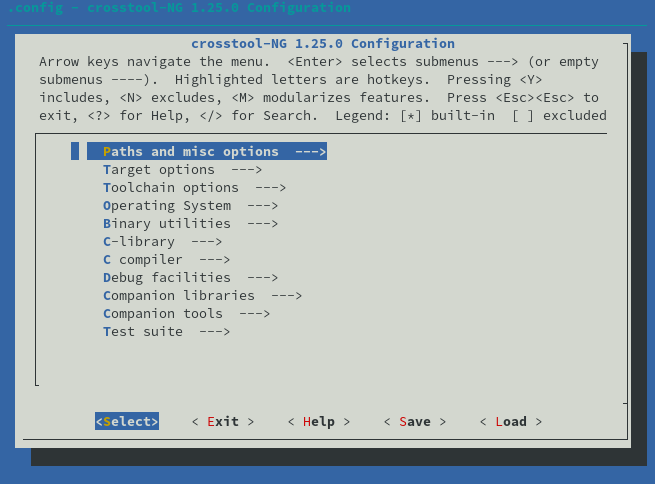
\includegraphics[width=\textwidth]{slides/sysdev-toolchains-obtaining/ct-ng-menu.png}
  \end{columns}
\end{frame}

\begin{frame}
\frametitle{Toolchain building utilities (3)}
Many root filesystem build systems also allow the construction of
a cross-compiling toolchain
\begin{itemize}
\item {\bf Buildroot}
  \begin{itemize}
  \item Makefile-based. Can build glibc, uClibc and musl based
    toolchains, for a wide range of architectures. Use \code{make sdk}
    to only generate a toolchain.
  \item \url{https://buildroot.org}
  \end{itemize}
\item {\bf PTXdist}
  \begin{itemize}
  \item Makefile-based, maintained mainly by {\em Pengutronix}. It only
        supports uClibc and glibc (version 2021.03 status)
  \item \url{https://www.ptxdist.org/}
  \end{itemize}
\item {\bf OpenEmbedded / Yocto Project}
  \begin{itemize}
  \item A featureful, but more complicated build system
  \item \url{http://www.openembedded.org/}
  \item \url{https://www.yoctoproject.org/}
  \end{itemize}
\end{itemize}
\end{frame}

\begin{frame}[fragile]
  \frametitle{Crosstool-NG: installation and usage}
  \begin{itemize}
  \item Installation of Crosstool-NG can be done system-wide, or just locally in
    the source directory. For local installation:
\begin{verbatim}
./configure --enable-local
make
make install
\end{verbatim}
  \item Some sample configurations for various architectures are
    available in
    samples, they can be listed using
\begin{verbatim}
./ct-ng list-samples
\end{verbatim}
  \item To load a sample configuration
\begin{verbatim}
./ct-ng <sample-name>
\end{verbatim}
  \item To adjust the configuration
\begin{verbatim}
./ct-ng menuconfig
\end{verbatim}
  \item To build the toolchain
\begin{verbatim}
./ct-ng build
\end{verbatim}
  \end{itemize}
\end{frame}

\begin{frame}
  \frametitle{Toolchain contents}
  \begin{itemize}
  \item The cross compilation tool binaries, in \code{bin/}
    \begin{itemize}
    \item This directory should be added to your \code{PATH} to ease
      usage of the toolchain
    \end{itemize}
  \item One or several {\em sysroot}, each containing
    \begin{itemize}
    \item The C library and related libraries, compiled for the target
    \item The C library headers and kernel headers
    \end{itemize}
  \item There is one {\em sysroot} for each variant: toolchains can be
    {\em multilib} if they have several copies of the C library for
    different configurations (for example: ARMv4T, ARMv5T, etc.)
    \begin{itemize}
    \item Old CodeSourcery ARM toolchains were multilib, the sysroots in:
      \code{arm-none-linux-gnueabi/libc/armv4t/}\\
      \code{arm-none-linux-gnueabi/libc/thumb2/}\\
    \item Crosstool-NG toolchains can be multilib too
      (\code{CT_MULTILIB} configuration parameter)
    \end{itemize}
  \end{itemize}
\end{frame}
